\chapter{Machine Learning}

\section{Introduction}
The world of today is generating huge amounts of data
as it goes along,
and more and more of it is put to use.
It is quite probable that any consumer in our society
that goes shopping,
uses some kind of service,
or uses the internet
on a daily basis
performs actions that end up in a database.
Not only do persons generate data,
so does everything else we monitor,
and our society happens to monitor quite a lot.
This data is invaluable for any organization that benefits
from information,
and truly, most do.
It is used by financial institutions like insurance companies,
medical institutions, commercial companies, scientific research
and everything in between.
Evidently, as the need for knowledge (or awareness thereof)
increases, so must our abilities to uncover it,
making machine learning an incredibly interesting topic
in today's world.

People are good at creating hypotheses
about what things mean,
connecting the dots
and predicting cause or outcome.
Yet we can only cope
with so much data at a time
and without direction,
the answers we seek may elude us.
Enter the computing device,
programmable to our needs.
Computer programs often take the form
of our expert knowledge put to detailed writing
but they can also cover the gaps where
we don't have the knowledge
and instead need to uncover it.
This includes anything of valuable information to us,
be it patterns in certain data or hypotheses for predictions.
Where the domain expert describes such hypotheses
using a computer program,
the machine learning expert devises ways of uncovering
the hypotheses.
Evidently, the power of computers would be much greater
if they would be made able to learn as we do.

Great advances have already been made in the domain,
yet we have not managed to make computers learn
as well as humans do,
at least not in as many regards as we do.
The best applications do, however,
get better results than humans in very specific domains.


\paragraph{}
Machine learning is a collection of methods
used to bridge the aforementioned gap
between data and knowledge.
A machine learning algorithm learns from data
and learns an hypothesis or model on it,
which can then be used to make predictions on future data.
This separates it from other algorithms
designed by an expert
that follow a static rule set.
It is inherently an interdisciplinary field,
with its roots firmly embedded
in a statistical foundation
combined with AI,
drawing inspiration from fields such as
information theory,
complexity theory,
psychology
and other fields.

The rest of this chapter will describe the basics of machine learning
along with the specific tools I will use throughout this thesis.
The foundation should be quite sufficient to build up
an understanding of the field
so as to allow the reader to follow the following chapters comfortably.
Next to exploring a foundation,
I will describe specific methods such as neural networks
and convolutional layers,
both exciting techniques that will be used further on.
However, perhaps to the reader's delight,
a cursory glance at the high-level introduction of these methods
should suffice for the reader who only seeks to understand
the applications described herein.
The careful reader is of course cordially invited
to read the more detailed descriptions.


\section{Hands-on Introduction}
A machine learning algorithm
is usually required to form hypotheses
based on given observations.
In this way it can be seen as
a black-box oracle
in which data are shoved
and answers pop out.
Let's take as an easy example
the probably overused and dead-beaten weather forecast.

Let's say we only need to do a daily forecast.
Data come in in the form of meteorological observations
such as temperature, wind speed, and whatever else
experts observe to make top-notch predictions.
This then gets paired
with a description of the actual weather the next day.
Together they form experience-target pairs
$(x_i, y_i)$
that correspond to a meteorological observation
on the one day and the weather on the next day,
in the hope that we can somehow deduce the hidden
link between the two.
The target $y_i$ is what we're really after
so we should choose carefully as to what we are trying to predict.
$y_i$ can be a nominal value,
i.e. from a given set of values
such as the set $(sunny, rainy, windy)$,
in which case the problem is called a \textit{classification} problem.
Contrarily, it can be a real-valued number such as temperature
in which case we call the problem a \textit{regression} problem.
The distinction is worth noting because
some techniques lend themselves well to
one category but not necessarily to the other.
On this data we will try to learn a hypothesis $h$
that can predict the target weather $y$
for any given observation $x$.
Now all we need to do is fill in the bits in between.

We already have a vague description of what we want to achieve
but now we need to design the problem.
Let us pick for our targets the real-valued temperature on a given day.
The observations, or \textit{features}, we will base our model on
will take the form of a vector
$(Temperature, Sky, Wind)$ or $(x_1, x_2, x_3)$ short,
where $Temperature$ and $Wind$ are real-valued,
whereas $Sky$ takes on one of the three values
$(Sunny, Rainy, Cloudy)$.
Now we need some kind of function connecting
observation to target.
One of the easiest choices would be a linear
function that combines the features
and outputs the target we are looking for.
It would look quite simple:

$$ y = w_0 + w_1x_1 + w_2x_2 + w_3x_3 $$

We are still stuck with the problem that $x_2$, or $Sky$,
is a nominal value and therefore does not fit all too well with algebra.
We can work around this by agreeing on
a little preprocessing step
that maps $Sunny$ to $-1$, $Rainy$ to $0$ and $Cloudy$ to $1$.
Now that our model is defined, all that is left for us to do
is train it.

In order to train our model we need a data set with training examples
$(x_i, y_i)$,
where the temperature $y_i$ corresponds to
the observations $x_i$ the previous day.
All that remains now is to pick the best weights
so the resulting model is the best hypothesis.
We describe a \textit{best fit}
we need some metric of performance.
The easiest one available is the error on the predictions made by the model
compared to the targets in the training data.
The best hypothesis is the one that minimizes this error.
The most common error by far is the \textit{mean squared error},
though others certainly exist.
Given a training set $D$, it is defined as follows:

$$ E = \frac{1}{|D|} \sum_{(x_i, y_i) \in D}{(h(x_i) - y_i)^2} $$

Multiple algorithms exist that minimize $E$ in such a manner.
If all data is available in one go, as it is in our case,
we can simply apply linear regression to our system
of $|D|$ equations $y = xw$ in order to find a $w$
with the lowest error.

\subsection{Finishing up the example}
An alternative algorithm to find our optimal weights $w$
is the \textit{weight update rule},
a source of inspiration for many more algorithms.
The idea behind is that every sample
you calculate your prediction
and shift the weights in the direction of the error,
proportionally to the size of the error.
So, for every sample:
\begin{enumerate}
\item Calculate $\hat{y_i} = h(x_i)$
\item Update $w_i = w_i + \eta(y_i - \hat{y_i})x_i$
\end{enumerate}

The update size can be tweaked with $\eta$.

\paragraph{}
As you have witnessed yourself,
designing a machine learning task
is rather an art than an exact science.
The first optimization algorithm proposed,
linear regression,
is only available for linear models.
Finding the ultimate weights
makes more sense in a regression context
as opposed to a classification context.

There are many more such decisions to made
and models to choose from.
During the next sections,
I will touch on some interesting
models that are used throughout this thesis.

\section{Underfitting and Overfitting}
Why not just go for an error of $0$?
We could, however it is unlikely since we suffer from two problems:
insufficient data and a delusion of a perfect world.
In other words, our features probably are not sufficient
and our data is noisy.
If we still manage a training error of $0$
we probably committed the grave mistake of
\textit{overfitting} the training data,
meaning we included the noise of the data in our model.
The reason this is to be avoided is that by definition
noise cannot be predicted and a model that tries
to do so will perform even worse on similar unseen samples.

\paragraph{}
Figure
\ref{fig:overfitting}
demonstrates this phenomenon of overfitting.
A high-dimensional polynomial is fitted on
a small set of samples drawn from a noisy
distribution that follows a goniometric function.
The model that we would like to attain
should be as close as possible to the original function.
However, if we try to fit the available data completely,
the polynomial results in a model that performs
well in the very close vicinity of the training points
but performs horrendously on unseen data
that deviates from the original training data.
This can be seen from the discrepancy
between the model and true function.
It follows that overfitting is characterized by
a low training error but a high generalization error,
or put otherwise,
the model fails to generalize the training data.

\begin{figure}[h]
\center
\begin{subfigure}{.49\textwidth}
  \centering
  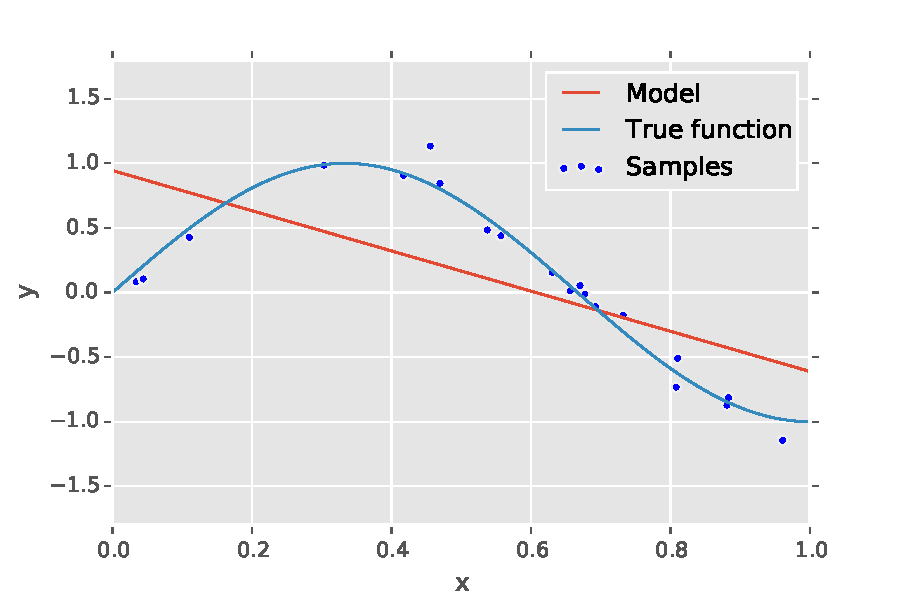
\includegraphics[width=\textwidth]{underfitting.pdf}
  \caption{Underfitting}
  \label{fig:underfitting}
\end{subfigure}
\begin{subfigure}{.49\textwidth}
  \centering
  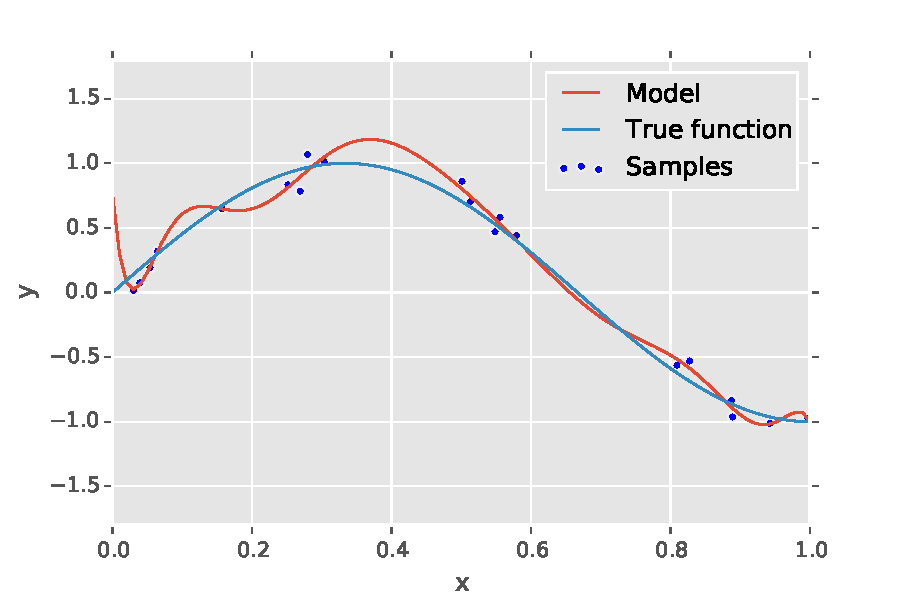
\includegraphics[width=\textwidth]{overfitting.pdf}
  \caption{Overfitting}
  \label{fig:overfitting}
\end{subfigure}

\label{fig:fitting}
\caption[Underfitting and Overfitting]{
Underfitting and overfitting
demonstrated with two polynomial
models on noisy data modeled
after a goniometric function.
}
\end{figure}

The opposite of overfitting would then be \textit{underfitting},
as demonstrated by Figure \ref{fig:underfitting}.
This is often the case for models that lack
representational power
no matter how much data is available.
While the figure contains a rather naive example
of a 1-dimensional polynomial fit,
it illustrates perfectly how some models
can never hope to attain a complex underlying function.

It will not be possible to minimize the training error entirely,
though an underfitting model may still outperform
an overfitted one.

\paragraph{}
As should be clear from the example,
neither under- nor overfitting are good,
in fact an algorithm designer
should be weary of both.
It is best to explore multiple
algorithm settings in order to find
a model that is prone to
neither kind of misfitting.

In the next section I will describe a measure
that helps guide this search.

\begin{figure}[h]
\center
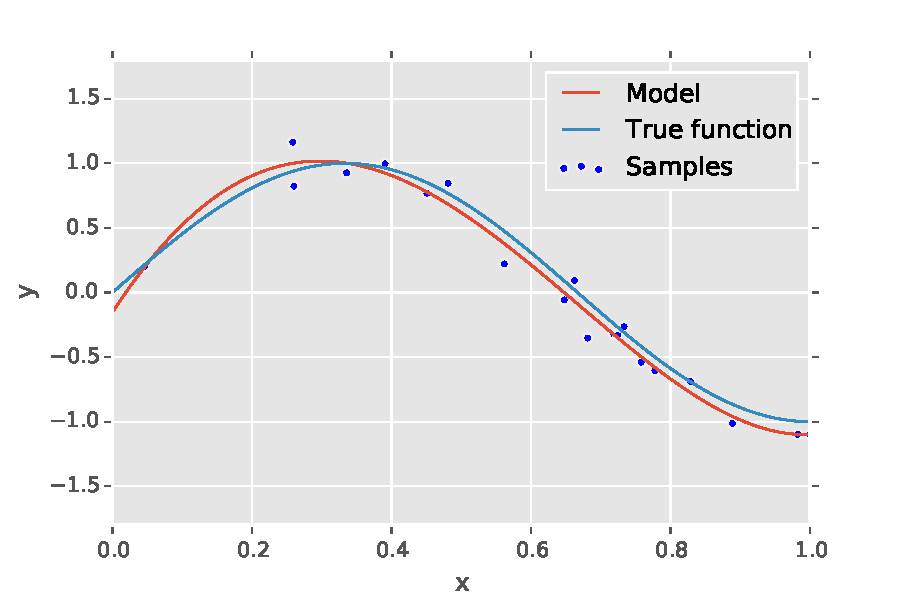
\includegraphics[width=.7\textwidth]{perfectfitting.pdf}
\label{fig:perfectfitting}
\caption[Curve fitting]{The right model can perfectly generalize from noisy data,
insofar as the data covers the desired domain}
\end{figure}

\section{Bias and Variance}
A common way to describe a learning algorithm
is in terms of its
bias and variance.
They are two different sources of error
the algorithm designer wishes to minimize.
The \textit{bias} of a learning algorithm
is the error inherent to the algorithm
because of false assumptions,
such as an unsuitable degree for a polynomial model
in the previous example.
This does not necessarily mean the model is weak on its own,
it only is for a specific problem.
Bias gives cause to underfitting,
as can be seen in Figure \ref{fig:underfitting}.

Bias can be quantified as the difference
between the expected prediction
and the true function value:

$$
\text{Bias}(x) = E[\hat{f} (x)] - f(x)
$$

\textit{Variance}
on the other hand,
is error because of sensitivity to noise:
small fluctuations in the data set.
It is the variability of a model's predictions.
As a result,
high variance may causes overfitting
noise inherent to the data but not to the model.
A typical example can be seen in Figure \ref{fig:overfitting}.

Variance can be quantified in terms of
the expected deviation of a prediction (variability):

$$
\text{Variance}(x) = E[ (\hat{f}(x) - E[\hat{f}(x)])^2]
$$

It can be lowered by
reducing the amount of features
(especially those of little import to the model)
or increasing the amount of data points.

\paragraph{}
Bringing these two notions together
gives us the \textit{bias-variance decomposition}
of a learning algorithm's generalization error,
i.e. the expected error on unseen data:

$$
\text{Err}(x) = E[(Y - \hat{f}(x))^2]
$$
$$
\text{Err}(x) = (E[\hat{f} (x)] - f(x))^2 + E[ (\hat{f}(x) - E[\hat{f}(x)])^2] + \sigma^2
$$

As you can see, the first two terms
are Bias squared and Variance respectively.
That leaves us with the last term
which is the irreducible error,
an error resulting from a lack of
omniscience; a lack of data.

From this decomposition we can see that we
can see that we can only have an error of 0
given the original model behind the data
an infinite amount of data. % bold claims man

\begin{figure}[ht]
\center
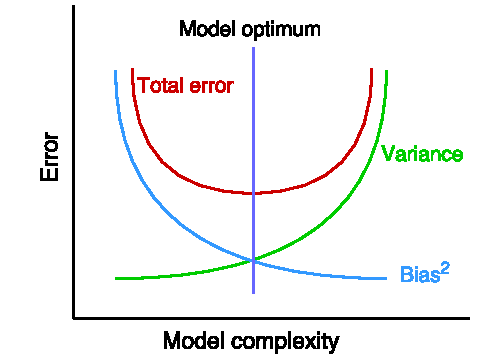
\includegraphics[width=0.7\textwidth]{bias_variance.pdf}

\caption{Bias-Variance decomposition}
\label{fig:biasvariance}
% TODO
\end{figure}

\paragraph{}
Figure \ref{fig:biasvariance}
visualizes the bias-variance decomposition
and shows the general tendencies of its individual components.
As bias decreases, variance generally goes up
and vice versa.
The goal of any algorithm designer
is then to find the sweet spot;
the model that optimizes the traded
between the two.

This can be done by exploring parameters
for a certain model,
like the degree of a polynomial,
and calculating the
\textit{expected generalization error}, % yes made this up myself lucid moment
since the true generalization error
is never known.
This in turn can be done
by keeping a separate test set
and calculating the error on that,
or other techniques that make clever use
of the training data
such as bootstrap or cross-fold validation.
I'll delve into those in the next section.

\begin{figure}
\center
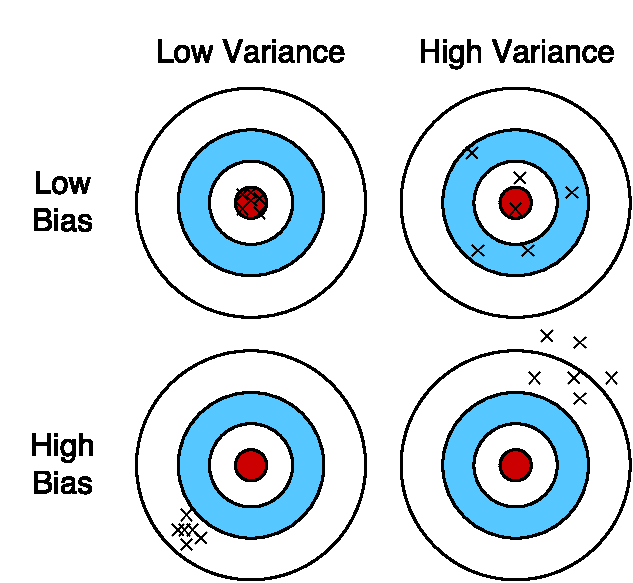
\includegraphics[width=0.7\textwidth]{dartboard.pdf}
\caption[Dartboard Analogy]{
  Dartboard Analogy
  \parencite{sammut2011encyclopedia}
}
\label{fig:bullseye}
\end{figure}

\paragraph{}
So far the discussion on the
generalization error and how to mitigate it,
I'd like to finish with a depiction
of bias and variance in Figure \ref{fig:bullseye}.
The center of the red target
is some target value $f(x)$
and darts are predictions $\hat{f}(x)$.
You can imagine this is the same x
for many instantiations of the same model
or it is a different x for every dart $\hat{f}(x)$,
it doesn't matter.

A high variance will have a scattering effect.
After all,
variance describes the variability of predictions.
High bias is the inability to generalize
well because of the model's false assumption:
in the image the model assumes an incorrect target.
The goal is once to have both measures as low as possible.

\section{Model Validation}
When training a model,
one typically wants to know the generalization error
as it is described in the previous section.
You already have the training error
because it is what you are trying to minimize,
but it usually generalizes poorly
to the generalization error.
It can actually be harmful to
watch only the training error during training,
so you need an indication of how the model
generalizes past training.

Often there are training, validation and test phases.
Validation is the stage
where we are trying to decide on the best model;
this is when model parameters are determined
(model selection).
During testing we simply see how well the model
is expected to generalize beyond experience.
At this point no more tuning is performed.
If the same data would be used for both validation
and testing,
the resulting test error
would probably be overly optimistic
\parencite{friedman2001elements}
since we are trying to determine prediction error
based on the data that was used to determine
the very model we are using.


\paragraph{}
A naive way to go about this
is to take a separate set of data
that comes from the same distribution
as the training data
(because otherwise your measure says very little
or your training data was chosen poorly)
and calculate the error of the model on this set.
This \textit{validation set} should be large enough
to be representative of the underlying distribution
but need not be as large as the original training set.
A common measure,
when dividing a data set,
is to keep 20\% to 30\% aside
for validation purposes.
If a test set is also required,
a good rule of thumb is keeping
50\% for training data
and dividing the other 50\%
equally over validation and test sets.

This way of splitting up data is far from ideal
because it requires that the validation data
not be used during training.
Data is however far too valuable for training,
we would rather not use it to simply
compute a measure of success.

\subsection{Cross-Validation}
Cross-validation or K-fold cross-validation
is by far the most popular validation technique.
Gone with the separate validation set
(I'll ignore testing for prediction error for now),
cross-validation testing solves
the problem of data scarcity by not using up
the data you desperately need for training.

\begin{figure}[h]
\center
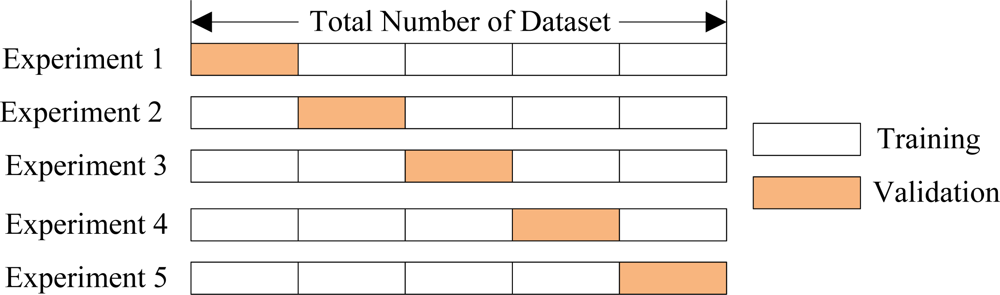
\includegraphics[width=0.8\textwidth]{crossval.png}
\caption[5-fold cross-validation]{
5-fold cross-validation
\parencite{Zhang2011}
}
\label{fig:crossval}
%TODO check attribution
\end{figure}

Figure \ref{fig:crossval} illustrates
how the training set is now divided into
K equal-sized \textit{folds}.
Each of these folds will be a validation set
in its own time.

The technique requires K
different models to be learned,
for a total of K iterations.
During iteration $i$,
fold $i$ is kept aside
as the validation set for this iteration
and all other folds together comprise
round $i$'s training set.

For each model the error is calculated on the validation
set, let's call this $\textit{CV}_i$.
The cross-validation error then becomes:

$$
CV(\hat{f}) = \frac{1}{N} \sum^{N}_{i=1} CV_i
$$

\paragraph{}
We now have a guess at the prediction error.
A good K is paramount for a good cross-validation error,
it also has a huge impact on the required amount of work
since computation time grows linearly with K.
We would like it to be quite low to save on computation time
yet high enough to have the cross-validation error
be a meaningful estimate.
Lower K tend to higher bias
because less data is used for training.
Higher K then tend towards
high variance.
This comes down to the same trade-off between
bias and variance,
though this time of an estimator
that estimates generalization error.
Generally good compromises for K are 5 and 10
\parencite{kohavi1995study}.

\section{Curse of Dimensionality}
The distance between two instances is calculated based on all of their attributes.
For these instances to have a small distance between them,
they should be close to one another in all of their attributes,
or otherwise put,
they should be similar in all aspects.
The more attributes or dimensions they have,
the harder this becomes.
This informally described phenomenon we call
the \textit{curse of dimensionality}.

\begin{figure}[ht]
\center

\begin{subfigure}{.49\textwidth}
  \centering
  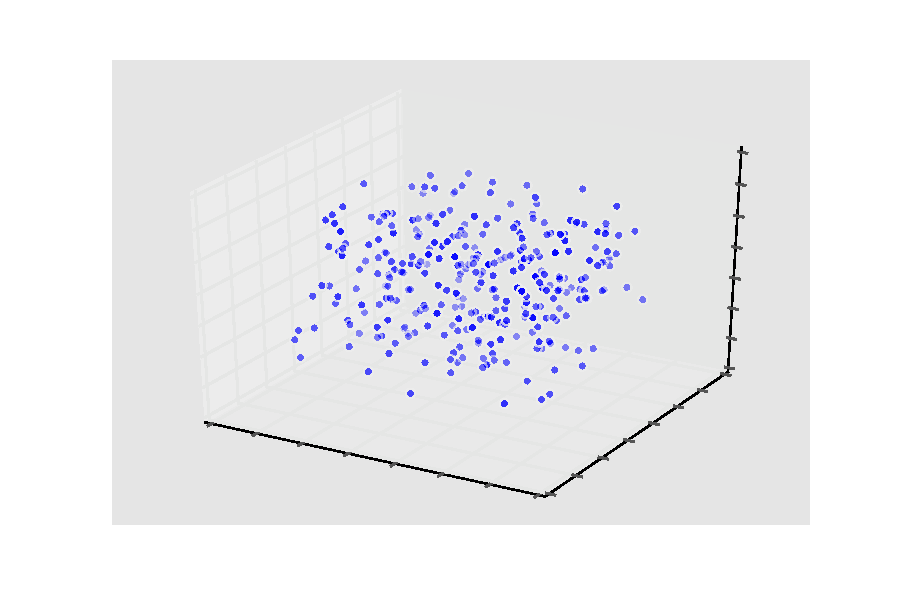
\includegraphics[width=\textwidth]{curse_3d.pdf}
  \caption{3 dimensions}
  \label{fig.ml.cod3}
\end{subfigure}
\begin{subfigure}{.49\textwidth}
  \centering
  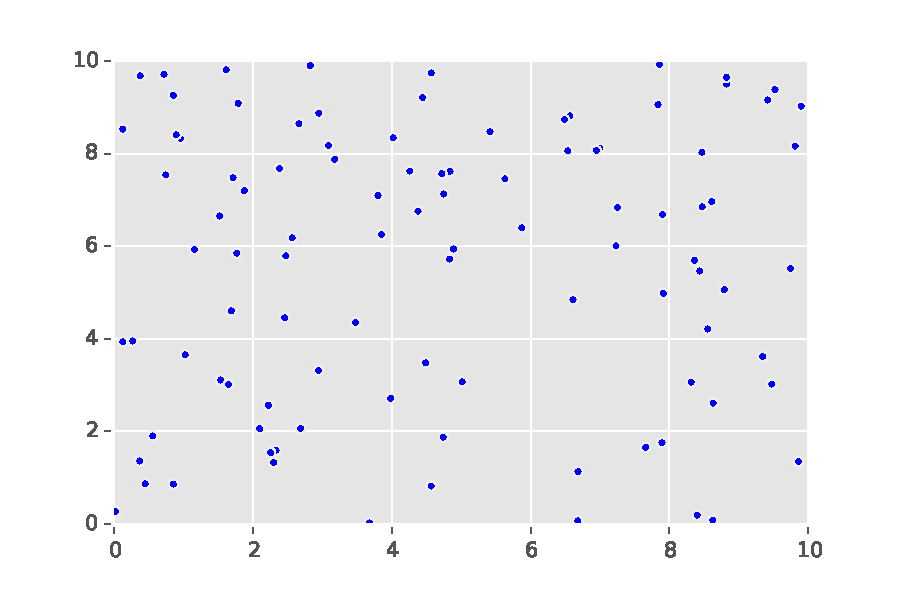
\includegraphics[width=\textwidth]{curse_2d.pdf}
  \caption{2 dimensions}
  \label{fig.ml.cod2}
\end{subfigure}
\begin{subfigure}{.45\textwidth}
  \centering
  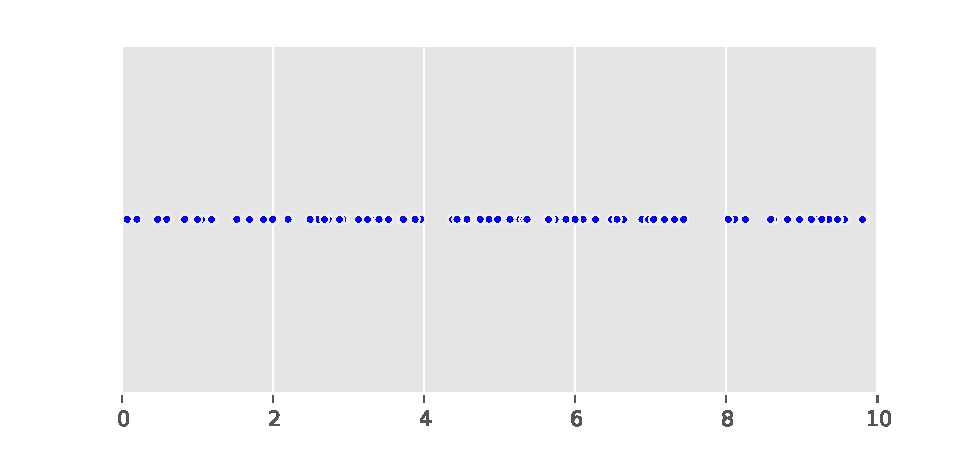
\includegraphics[width=\textwidth]{curse_1d.pdf}
  \caption{1 dimension}
  \label{fig.ml.cod1}
\end{subfigure}

\caption[Curse of dimensionality]{Each plot contains 100 points
with values in all dimensions ranging
uniformly between 0 and 10.
The curse of dimensionality is especially clear
from the difference between the 2-dimensional
and 1-dimensional plot.
}
\label{fig.ml.cod}
\end{figure}

Figure ~\ref{fig.ml.cod} attempts a visual demonstration.
Each plot contains 100 instances with a variable amount of dimensions,
but with values for all dimensions ranging uniformly between 0 and 10.
As instances gain more dimensions,
the spaces containing them become increasingly more sparse.
Even though an instance may be close to another instance
in some dimensions,
any discrepancies in other dimensions
will only increase the distance between the two instances.

Let us resume with the above example.
Another way to uncover the increasing sparsity is to examine
is by examining the density of each space.
The 1-dimensional space has 10 instances per unit of space,
since it contains 100 instances spread over 10 units.
In contrast then, the 2-dimensional space contains
only a single instance per square unit of space
and the 3-dimensional space a forlorn $.1$ instance
per cubic unit of space.
In order to boost the density of the 3-dimensional space
to be on par with the 1-dimensional one,
we would need a hundred times as many instances
in this particular scenario,
for that is the factor between the two space sizes.

A final measure of sparsity of a space I like to think in
is the expected average distance for dimensions,
given their distributions.
In other words,
if one were to pick two instances from one of the above spaces uniformly,
what would the expected distance between the two be?
This measure relates directly to the curse of dimensionality;
as the number of dimensions increase,
expect the distances to go up as well.

\paragraph{}
The phenomenon is often encountered in areas such as
text processing or image processing
where large numbers of dimensions are inevitable.
A naive model that tries to represent texts
could have a different dimension for each word,
likewise a model that describes an image
would have a separate dimension for each pixel,
easily reaching into thousands of attributes.

Such models would need a tremendous amount
of instances to have any sort of meaningful
distance measure.
Acquiring the required quantities of data
is often infeasible,
making techniques that shrink space dimensionality
very valuable in practice.
Techniques can range from discarding
least important attributes to
statistically combining attributes
to even learning new attributes that represent
higher-level concepts
from the lower-level attributes.
A popular example of the latter are
convolutional networks,
a topic I will cover in
section \ref{sec:cnn}.

